\section{Analysis and Results}
\label{sec:analysis}
\subsection{Single Player}
While Talker did effectively communicate board conditions, it was never tested extensively.  Instead, we focused singleplayer testing on PatternMaker.  Some of the results are shown in the table below:
\TODO{[RESULTS TABLE, TO BE GENERATED]}

\subsection{Multi-player}
Note that our submitted multi-player strategy is focused specifically on the default setup.
A few reasons are listed below.
\begin{enumerate}
  \item We believe there is no single strategy that can outperform others in both single player and multi-player case. The tournament result strongly supported this. The player perform well in single mode are easily died in multi-player case.
  \item We do not want to design an algorithm that performs ok in all set up but not be able to win any of them.
  \item We are really interested in multi-player mode. 
  As mentioned in the previous section, in fact, our single player strategy can outperform the results in tournament, both abundant resource and spareness case, in terms of average sustainable energy. We decide to submit multi-player strategy simply because it is more fun to watch our organism flooding others.
\end{enumerate}

Quote from the tournament result:

\textbf{Multi-player, [X=20, Y=20, p=0.01, q=0.02, maxrounds=50000]:}
\begin{verbatim}
                Average End Energy	Average Extinction
Group1PlayerNew 0                   (2,755)
Group2Player    0                   (4,498)
ShyPlayer       0                   (3,047)
RainbowCastle   29,651              (2,486)
Group5Flood     19,362              (6,258)
Group6Player    0                   (1,612)
\end{verbatim}
The only enemy that survives with flood is \textit{RainbowCastle} from group 4.
We have lower average energy than them, but our average Extinction is much longer than
they have, which means if they die, they will die really early in the game.
Here is a detailed look of the ten trails stats of the two group:
\begin{verbatim}
RainbowCastle 27,989    (2,362)  (2,798)  29,812   28,184   
              (1,069)   (2,182)  32,620   (2,218)  (4,284) 
Group5Flood   (13,959)  16,931   18,955   (3,054)  (3,808)
              17,675    20,226   (1,156)   23,187  19,196 
\end{verbatim}
As one can see, RainbowCastle extinct for six times which we only extinct for four, 
which make us question the meaningfulness of the given stats.
Essentially, if extinct, the end energy is zero.
If not extinct, the Extinction time will equals the maxrounds
(assume world is doomed at the last round and all organisms are slaughtered).
We recalculate the final stats and get the following:
\begin{verbatim}
                Average End Energy	Average Extinction
RainbowCastle   11860              (21491)
Group5Flood     11617              (32503)
\end{verbatim}
Now, one can see that the average end energy are almost the same but our average extinction 
is much later.
The reason for this is that we are not performing any energy maximization in the multi-player case. As discussed before, the ecosystem will always force the family to expand if having extra energy.
If making an analogy to boxing, our player is always aiming at knocking out instead of earning more technical score.
Nevertheless, extinct two times less out of ten trail might not be sufficient to demonstrate the power of our player. 
We are looking forward to do a bit more test if having their class file.

\textbf{Multi-player, [X=20, Y=20, p=0.01, q=0.02, maxrounds=50000]:}
\begin{verbatim}
                Average End Energy	Average Extinction
Group1PlayerNew   0                  (3,493)
Group2Player      0                  (9,740)
ShyPlayer         0                  (4,190)
RainbowCastle     0                  (13,715)
Group5Flood       119,438            N/A
Group6Player      0                  (5,283)
\end{verbatim}
We overwhelmingly win the game under this setup.
One of the reason might be the expanding nature of our ecosystem.
The larger the board, the more space the whole family have to flood.

\textbf{Additional setup: 1 flood vs 4 sheep, [X=20, Y=20, p=0.01, q=0.02, maxrounds=20000]}
\begin{verbatim}
[Player Configuration]:
	[Player0]: Flood
	[Player1]: Summer 2012 Player
	[Player2]: Summer 2012 Player
	[Player3]: Summer 2012 Player
	[Player4]: Summer 2012 Player
[SUMMARY of 10 trials]
Player: 0 Mean Count: 110 Mean Energy: 13163 Extinction: 3
Player: 1 Mean Count: 18 Mean Energy: 3230 Extinction: 9
Player: 2 Mean Count: 12 Mean Energy: 2470 Extinction: 9
Player: 3 Mean Count: 0 Mean Energy: 0 Extinction: 10
Player: 4 Mean Count: 24 Mean Energy: 4265 Extinction: 8
\end{verbatim}

\begin{figure}[ht]
\centering
  % Requires \usepackage{graphicx}
  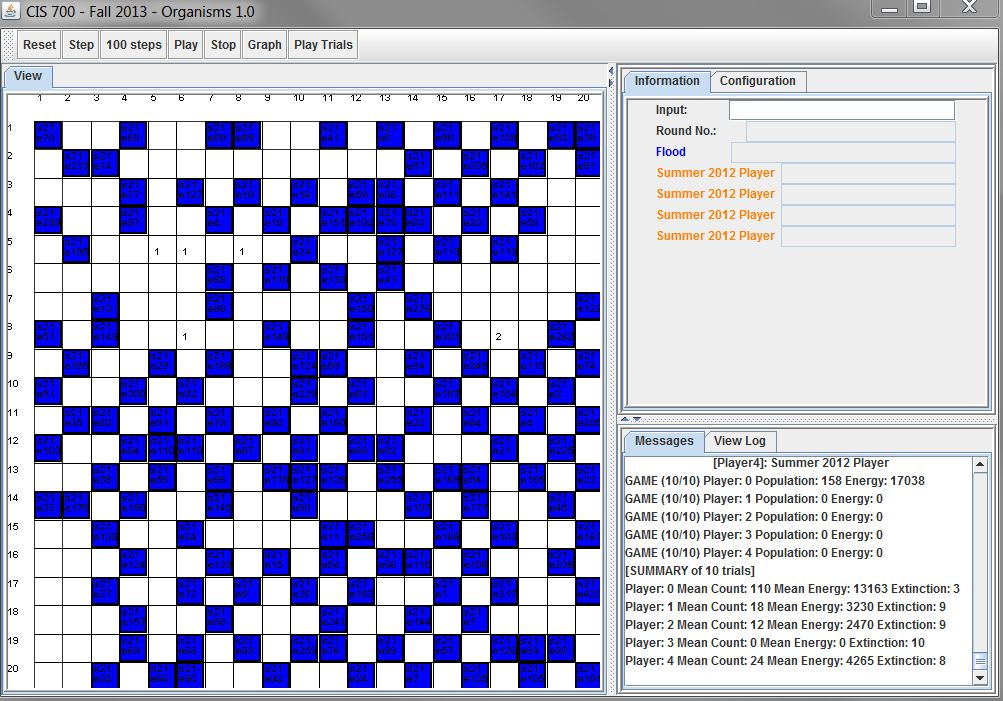
\includegraphics[width=150mm]{figs/1v4.JPG}\\
  \caption{Screen shot of 1 food vs 4 sheep}\label{fig:1v4}
\end{figure}

One can see that we still win(extinct all sheep) 70\% of time.
Note that sheep is not communication based strategy, thus putting multiple 
sheep on the board will only increase the initial energy the expanding rate 
of sheep instead of having two sheep realm and fighting with each other.
